\part{Further results and a constructive optimization method}

The results in this part extend the resolution in Part~I. Publication priority has not been established. Each use of the general classification is stated explicitly. Several of the new statements are separately formalized in Lean, as recorded in Appendix~\ref{app:formal}.

\section{The complete order theory of the original example family}

The family $W_p$ in \eqref{eq:Wp} is a useful laboratory because its detection order is exactly solvable while its ellipsoid loses orientation information. The family itself is from Example 2 of \cite{milne}. The following results quantify over all complex density matrices, not only Bell-diagonal states.

\begin{theorem}[Exact detection order]\label{thm:parametric-order}
For $0<p,q\leq1$,
\[
 D(W_p)\subseteq D(W_q)\iff p\leq q,
 \qquad D(W_p)\subsetneq D(W_q)\iff p<q.
\]
For $q>0$, the complete scalar subtraction criterion is
\[
 W_p-\alpha W_q\succeq0
 \iff \alpha=p/q\ \text{and}\ p\leq q,
 \qquad p,\alpha\in\R.
\]
\end{theorem}
\begin{proof}
The identity
\[
 qW_p=pW_q+(q-p)P_+
\]
gives the positive-remainder comparison for $0<p\leq q$. Define the density matrix
\[
 \rho_t=\frac12\begin{pmatrix}
 0&0&0&0\\0&1&t-1&0\\0&t-1&1&0\\0&0&0&0
 \end{pmatrix},\qquad 0\leq t\leq2.
\]
Its nonzero eigenvalues are $t/2$ and $1-t/2$, and
\begin{equation}\label{eq:universal-separator}
 \tr(W_r\rho_t)=\frac{t-r}{2}.
\end{equation}
Taking $t=p$ proves strictness when $p<q$; reversing the roles rules out the opposite order.

For the last assertion, the quadratic forms of $W_p-\alpha W_q$ on $\ket{00}$ and the unnormalized singlet $(0,1,-1,0)^{\mathsf T}$ are $(p-\alpha q)/2$ and $-p+\alpha q$. Positivity forces $p=\alpha q$. The remainder is then $(1-\alpha)P_+$, positive exactly when $p\leq q$.
\end{proof}

\begin{proposition}[Largest simultaneous separation margin]\label{prop:margin}
For $0\leq p<q\leq1$, the largest number $m$ for which one density matrix can satisfy
\[
 \tr(W_p\rho)\geq m,\qquad \tr(W_q\rho)\leq-m
\]
is $m=(q-p)/4$. It is attained by $\rho_{(p+q)/2}$.
\end{proposition}
\begin{proof}
The diagonal matrix $W_p-W_q$ has largest eigenvalue $(q-p)/2$. Thus the two inequalities imply $2m\leq\tr((W_p-W_q)\rho)\leq(q-p)/2$. Equation~\eqref{eq:universal-separator} gives equality at the stated state.
\end{proof}

\begin{theorem}[Exact geometric order]\label{thm:parametric-geometry}
For every real $p,q$,
\begin{align*}
 \E(W_p)\subseteq\E(W_q)&\iff |2p-1|\leq|2q-1|,\\
 \E(W_p)=\E(W_q)&\iff p=q\ \text{or}\ p+q=1.
\end{align*}
These equalities refer to the canonical affine images of the unit ball; for $0<p,q\leq1$ these are actual witness ellipsoids.
\end{theorem}
\begin{proof}
The maps are $(u_1,u_2,u_3)\mapsto(u_1,u_2,(2p-1)u_3)$. Necessity follows by testing the third-axis endpoint. For sufficiency, rescale the third preimage coordinate by $(2p-1)/(2q-1)$; its absolute value is at most one. If $2q-1=0$, the inequality also makes $2p-1=0$, so the zero-denominator case is immediate. Equality is equivalent to equality of the absolute values, which gives the two stated possibilities.
\end{proof}

Consequently, detection improves while the ellipsoid strictly shrinks on $0<p<q\leq1/2$. It improves while the ellipsoid strictly grows on $1/2\leq p<q\leq1$. Every $0<p<1/2$ supplies an equal-ellipsoid Class D counterexample $(W_p,W_{1-p})$. The planar transition is $p=1/2$, not a missing limiting case.

For a target with semiaxes $(1,1,r)$, $0\leq r\leq1$, the feasible members of this family have
\[
 (1-r)/2\leq p\leq(1+r)/2,\qquad p>0.
\]
The unique optimal member \emph{within this displayed family} is $W_{(1+r)/2}$. This restricted-family statement has a direct Lean proof. Optimality against every two-qubit witness is the separate general theorem proved in Part~I.

\begin{figure}[htbp]
\centering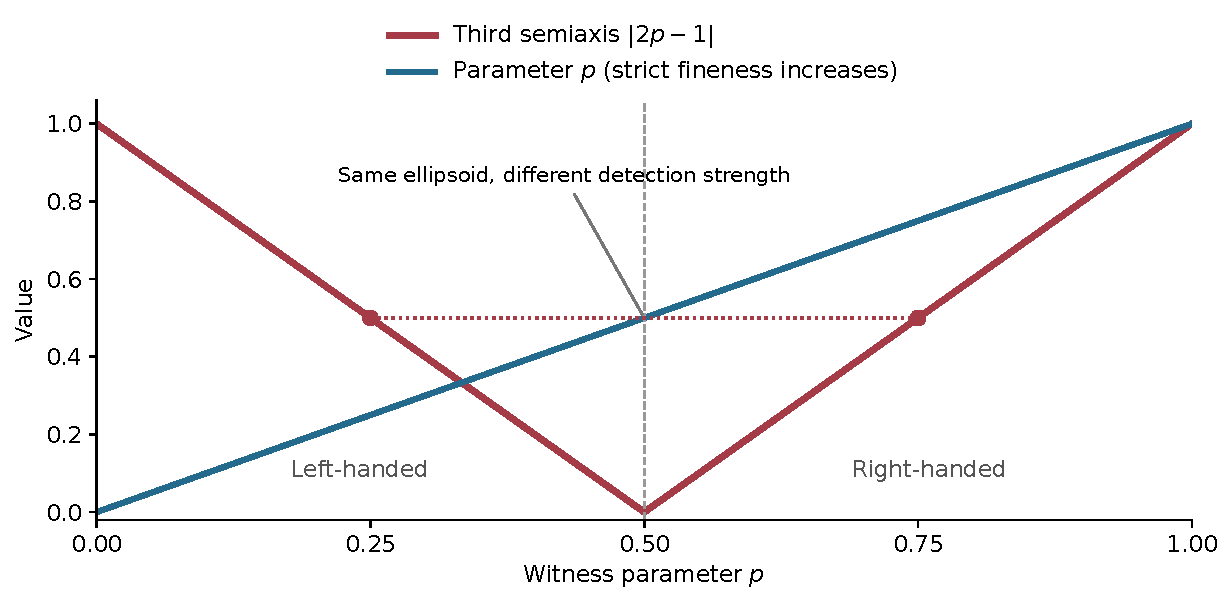
\includegraphics[width=.92\linewidth]{figures/parameter_orders.pdf}
\caption{The two orders for $W_p$. Fineness increases with $p$ throughout the witness interval. The third semiaxis, $|2p-1|$, decreases to zero and then increases. The mirror parameters $p$ and $1-p$ have identical filled ellipsoids.}
\end{figure}

\section{An exact convex program with a unique rank-one optimizer}

The refinement construction can be converted into a practical optimization problem. Fix the positive trace-preserving map $L$ associated with the target as in \eqref{eq:L}, and define the real-linear map on Hermitian matrices
\[
 M(Q)=(L\otimes\id)(Q^\Gamma).
\]
Although $M$ need not be positive on all bipartite positive operators, it maps every positive product operator to a positive operator. It preserves trace.

\begin{theorem}[Unique trace-minimizing refinement]\label{thm:sdp}
For $W\in\Sstar$, consider
\begin{equation}\label{eq:sdp-primal}
 \alpha_*(W)=\min_Q\tr Q,
 \qquad Q\succeq0,\qquad W-M(Q)\succeq0.
\end{equation}
This semidefinite program is feasible, attains its minimum, and has a unique minimizer $Q_*$. Moreover
\begin{enumerate}[label=(\roman*)]
\item $0<\alpha_*(W)\leq1$;
\item $Q_*=qq^\dagger$ for a nonzero entangled vector $q$;
\item $U_*=M(Q_*)/\alpha_*(W)$ is optimal in $\Sstar$;
\item $W=\alpha_*(W)U_*+P_*$, where $P_*\succeq0$ is singular;
\item $\alpha_*(W)=1$ if and only if $W$ is already optimal in $\Sstar$.
\end{enumerate}
The program has sixteen real variables and two Hermitian $4\times4$ positive semidefinite constraints. No rank constraint is imposed.
\end{theorem}
\begin{proof}
Part~I supplies a feasible $Q$. Trace preservation implies $0\leq\tr Q\leq1$. Thus the feasible set is closed and bounded inside the positive semidefinite cone, hence compact. A minimum exists and cannot be zero: a positive matrix of zero trace is zero, and $Q=0$ would require $W\succeq0$.

Suppose a minimizer has rank at least two. Choose a nonzero product vector $v$ in its range and set
\[
 \tau=(v^\dagger Q^+v)^{-1}>0,\qquad Q'=Q-\tau vv^\dagger\succeq0.
\]
Since $M(vv^\dagger)\succeq0$,
\[
 W-M(Q')=W-M(Q)+\tau M(vv^\dagger)\succeq0.
\]
This is feasible and has strictly smaller trace, a contradiction. Thus every minimizer has rank one. Its vector must be entangled, since a product vector would make both terms in $W=M(Q)+P$ positive. Its image is a witness with the whole target ellipsoid and the required chirality, and is optimal by Theorem~\ref{thm:main}.

If two distinct minimizers existed, their average would also minimize the objective. Two rank-one positive operators of equal trace and equal range are identical. Distinct minimizers therefore have different ranges, and their average has rank two, contradicting the preceding paragraph. This proves uniqueness.

If $P_*\succ0$, decreasing $Q_*$ by a sufficiently small positive scalar factor would keep the residual positive and decrease the objective. Hence $P_*$ is singular. Finally $\tr P_*=1-\alpha_*$; the fineness criterion proves the last equivalence.
\end{proof}

The rank-one and uniqueness argument is more general: it applies whenever the program is feasible for a nonpositive-semidefinite $W$ and a positive trace-preserving qubit map $L$. Geometric containment is a sufficient condition for feasibility furnished by Part~I; it is not a necessary condition. The examples below distinguish these statements.

Uniqueness here concerns the refinement selected by \emph{minimum trace}. It does not say that there is only one optimal witness in $\Sstar$, or only one optimal witness finer than a given $W$. Minimizing $\alpha$ maximizes the trace of the removable positive remainder.

\subsection{Dual certificates and exact arithmetic}

With the real Hilbert--Schmidt pairing on Hermitian matrices,
\[
 M^*(X)=\Gamma_B((L^*\otimes\id)(X)).
\]
The dual program is
\begin{equation}\label{eq:sdp-dual}
 \sup_X-\tr(XW),\qquad X\succeq0,\qquad I_4+M^*(X)\succeq0.
\end{equation}
Its sign can be checked without convention-dependent duality rules. For feasible $Q,X$,
\begin{equation}\label{eq:duality-gap}
 \tr Q+\tr(XW)
 =\tr((I+M^*(X))Q)+\tr(X(W-M(Q)))\geq0.
\end{equation}
Thus matching primal and dual values certify exact optimality. Since $M$ preserves trace, $M^*(I)=I$, and $X=\varepsilon I$, $\varepsilon>0$, is strictly dual feasible. Standard semidefinite duality gives zero duality gap \cite{boyd}. This does not by itself assert dual attainment on every boundary instance; primal attainment was proved separately by compactness.

The package includes a numerical solver and exact rational primal--dual examples. Numerical eigenvalue tolerances are reported as diagnostics, not as proofs. For rational examples the independent SymPy verifier checks the residuals and objectives exactly. For arbitrary real-algebraic input, real closed field quantifier elimination gives an exact finite procedure in principle; no practical complexity or numerical conditioning guarantee is claimed.

\subsection{A distinct affine SDP for containment itself}

The exact positive lift and two-qubit decomposability also give a finite convex test for containment. With $L$ fixed by the target and $\|b_W\|<1$,
\begin{equation}\label{eq:containment-sdp}
 \boxed{\E(W)\subseteq\E_*
 \iff \exists P,Q\succeq0:\quad
 W=(L\otimes\id)(P+Q^\Gamma).}
\end{equation}
The forward implication lifts $W$ to a block-positive $V$ and decomposes it. Conversely, $P+Q^\Gamma$ is block positive, has the same Bob marginal as $W$, and its conditional Alice vectors are in the unit ball. Applying $L$ sends them into $\E_*$. Trace preservation also implies $\tr P+\tr Q=1$.

This is an affine semidefinite feasibility problem with two positive $4\times4$ auxiliary matrices, so the containment region is a spectrahedral shadow. It works for singular targets: the linear equality automatically enforces their support restrictions. It uses the two-qubit decomposability theorem, whereas the smaller S-lemma certificate uses a quadratic constraint and one scalar multiplier.

The placement of the positive remainder is different in the two programs:
\begin{center}
\begin{tabularx}{\linewidth}{@{}l X@{}}
\toprule
Question & Exact constraint\\
\midrule
Containment & $W=(L\otimes\id)(P)+M(Q)$, with $P,Q\succeq0$.\\
Refinement & $W=R+M(Q)$, with $R,Q\succeq0$.\\
\bottomrule
\end{tabularx}
\end{center}
For Class D, $(L\otimes\id)(P)$ can be a witness. For example, with target $\operatorname{diag}(1,1,1/2)$ and $W=W_{1/4}$, the containment certificate is $P=\proj{\psi^+}$, $Q=0$, while the optimal refinement certificate is $Q=\proj{\phi^+}/3$, $R=2\proj{\psi^+}/3$.

For a rank-two target, choose $L\circ\mathsf T=L$. Then $(L\otimes\id)(P)=M(P^{\mathsf T})$, so \eqref{eq:containment-sdp} simplifies further:
\[
 \E(W)\subseteq\E_*
 \iff W=M(Q)\ \text{for some }Q\succeq0,\ \tr Q=1,
\]
under the same positive-definite Bob marginal hypothesis. Thus the normalized planar containment region, including positive operators, is the image of the density-matrix set, restricted to positive definite Bob marginals. Taking its closure adds the corresponding product-state limits. This strengthens the planar argument without using an inverse of the singular shape matrix.

\section{Sharp comparison of diagonal Class D mirrors}

Consider
\[
 W_\pm=\tfrac14(\II+a\XX+b\YY\pm c\ZZ),
 \quad 1\geq a\geq b\geq c>0,\quad a+b>1+c.
\]
Both are Class D and share semiaxes $(a,b,c)$. Set
\[
 d=a+b-1>c,\qquad t=1-a+b\geq d,
 \qquad \alpha_-=\frac{d-c}{d+c},\quad\alpha_+=\frac{t-c}{t+c}.
\]

\begin{theorem}[The complete feasible scalar interval]\label{thm:sharp-mirror}
For every real $\alpha$,
\begin{equation}\label{eq:sharp-interval}
 W_--\alpha W_+\succeq0
 \quad\Longleftrightarrow\quad
 \alpha_-\leq\alpha\leq\alpha_+.
\end{equation}
This interval is contained in $(0,1)$, and its width is
\[
 \alpha_+-\alpha_-=\frac{4c(1-a)}{(t+c)(d+c)}.
\]
If $a<1$, every interior coefficient gives a positive definite remainder.
\end{theorem}
\begin{proof}
Use the Bell basis $(\phi^+,\phi^-,\psi^+,\psi^-)$. The $\psi^-$ eigenvalue of the difference forces $\alpha\geq\alpha_-$, while its $\phi^-$ eigenvalue forces $\alpha\leq\alpha_+$. On that interval, the $\phi^+$ eigenvalue exceeds the $\phi^-$ eigenvalue by $(a-b)(1-\alpha)/2\geq0$. The $\psi^+$ eigenvalue is $[(1+a+b)(1-\alpha)+c(1+\alpha)]/4>0$. These are all four eigenvalues. The width follows by common denominators. When the interval has nonzero width and both bounds are strict, all four eigenvalues are positive.
\end{proof}

For the target map with Bloch matrix $\operatorname{diag}(a,b,c)$, the solution of \eqref{eq:sdp-primal} for $W_-$ is exactly
\[
 Q_*=\alpha_-\proj{\phi^+},\qquad U_*=W_+.
\]
An exact dual certificate is $X_*=4\proj{\psi^-}/(d+c)$. The eigenvalues of $I+M^*(X_*)$, in Bell order, are
\[
 0,\quad \frac{2(a+b)}{d+c},\quad \frac{2(b+c)}{d+c},\quad \frac{2(a+c)}{d+c}.
\]
They are nonnegative and $-\tr(X_*W_-)=\alpha_-$. This proves global SDP optimality, not merely the scalar comparison of a fixed pair.

A uniform detection separator for this entire family is
\[
 \rho=\frac{1+a+b}{2(a+b)}\proj{\psi^-}
       +\frac{a+b-1}{2(a+b)}\proj{\psi^+}.
\]
Its expectations are $\tr(\rho W_-)=c/4$ and $\tr(\rho W_+)=-c/4$.

For the original family and an outer canonical representative $W_q$, where $1/2\leq q\leq1$ and $0<p\leq q$, the corresponding exact certificates simplify to
\[
 Q_*=(p/q)\proj{\phi^+},\qquad X_*=(2/q)\proj{\psi^-},\qquad\alpha_*=p/q.
\]
This remains feasible for $p<1-q$, even though $\E(W_p)$ is then \emph{not} contained in $\E(W_q)$. Hence feasibility of the refinement SDP is strictly weaker than geometric containment.

\section{Counterexamples form an open set}

\begin{theorem}[A quantitative robustness ball]\label{thm:robust}
Define
\[
 H_-=\tfrac14(\II+\tfrac34\XX+\tfrac34\YY-\tfrac14\ZZ),
 \qquad J(W)=(I\otimes X)W^\Gamma(I\otimes X).
\]
For every Hermitian trace-zero $\Delta$ with $\|\Delta\|_F<1/48$, the matrices
\[
 W=H_-+\Delta,\qquad U=J(W)
\]
are trace-one Class D witnesses, have exactly the same ellipsoid, and satisfy $W-U/2\succ0$. Thus every such $W$ is nonoptimal in the set defined by its own ellipsoid.
\end{theorem}
\begin{proof}
The map $J$ preserves trace, Hermiticity, block positivity and the geometric ellipsoid: partial transpose and a Bob unitary only reparametrize the allowed Bob effects. It is an isometry for the Frobenius norm. At the centre, $J(H_-)=H_+$ and
\[
 \operatorname{spec}(H_--H_+/2)=\{1/32,1/32,1/32,13/32\}.
\]
Every normalized product expectation of $H_-$ is at least $1/16$. Since $\|\Delta\|_{\mathrm{op}}\leq\|\Delta\|_F<1/48$, block positivity persists with a strictly positive margin. The negative eigenvalues of $H_-$ and $H_+$ are $-1/16$ and $-3/16$. Testing their original eigenvectors shows that $W$ and $U$ remain nonpositive-semidefinite. Since $U$ is unitarily equivalent to $W^\Gamma$, the Class D conclusion follows.

Finally,
\[
 \|\Delta-J(\Delta)/2\|_{\mathrm{op}}
 \leq\tfrac32\|\Delta\|_F<1/32.
\]
This is smaller than the least eigenvalue of the original remainder, so $W-U/2$ is positive definite. The fineness criterion gives strict improvement.
\end{proof}

This is an open ball in the fifteen-dimensional real affine space of trace-one Hermitian matrices. The enclosing ellipsoid varies with $\Delta$; the theorem does not claim that one fixed ellipsoid serves the entire ball. Its purpose is to show that the failure is stable under arbitrary sufficiently small matrix perturbations, including nondiagonal ones.

\section{Convexity and arbitrarily close improvements}

\subsection{A second exact containment criterion}

The support function of the target is
\[
 h_*(n)=n\cdot c_*+\sqrt{n^{\mathsf T}Q_*n}.
\]
For trace-one Hermitian Bloch data with $\|b\|<1$,
\begin{equation}\label{eq:support-containment}
 \boxed{\E(W)\subseteq\E_*
 \iff n\cdot a+\|T^{\mathsf T}n-h_*(n)b\|\leq h_*(n)
 \quad\text{for every }n\in S^2.}
\end{equation}
Indeed, containment is equivalent to $n\cdot r_W(u)\leq h_*(n)$ for every $n,u$. Multiply by the strictly positive denominator and maximize the resulting linear function of $u$ over the unit ball. The maximum is the Euclidean norm in \eqref{eq:support-containment}. The argument works for flat targets as well as solid ones.

For each fixed $n$, this is a second-order-cone constraint affine in the original Bloch coefficients. Thus the region of trace-one Hermitian operators with positive definite Bob marginal and ellipsoid inside $\E_*$ is convex. If $\E_*\subseteq\B$, membership already implies block positivity. The nonpositive-semidefinite condition defining witnesses need not itself define a convex set; the following comparable segments are witnesses throughout.

\begin{theorem}[Arbitrarily close improvements]\label{thm:local}
Every nonoptimal member of $\Sstar$ has arbitrarily close feasible strict improvements. If $\chi(W)<0$, those improvements can be chosen to have negative chirality. Therefore the nonempty left-handed sector of $\Sstar$ has no maximal elements, even when comparisons are restricted to that sector.
\end{theorem}
\begin{proof}
Choose an outer optimal refinement $W=\alpha U+P$ with $0<\alpha<1$ and nonzero $P\succeq0$. For $0<t\leq1$, put
\[
 V_t=(1-t)W+tU,\qquad k_t=\alpha+(1-\alpha)t,
 \qquad\beta_t=\alpha/k_t.
\]
Then
\begin{equation}\label{eq:interpolation}
 W=\beta_tV_t+(t/k_t)P.
\end{equation}
This gives strict fineness for every $t>0$. A state detected by $W$ is also detected by $U$, and hence by their mixture; thus $V_t$ is a witness. The conditional Alice vector of $V_t$ is a positive weighted convex combination of the corresponding vectors for $W$ and $U$, so its ellipsoid remains inside $\E_*$. Equivalently, use \eqref{eq:support-containment}.

The family converges to $W$ in every matrix norm. If $\det\Theta_W<0$, continuity preserves that strict sign for all sufficiently small positive $t$. The main theorem excludes negative-chirality optimal witnesses, so the result applies to every member of the left-handed sector.
\end{proof}

This strengthens the earlier same-chirality example into a statement about every left-handed witness in every admissible enclosure. It also identifies local and global relative optimality: a nonoptimal point cannot be protected by restricting attention to a sufficiently small neighbourhood.

There is a stronger geometric version. For a left-handed $W$, apply the mirror lemma at its own ellipsoid, choosing $U$ with $\E(U)=\E(W)$. The same interpolation then satisfies $\E(V_t)\subseteq\E(W)$. For sufficiently small positive $t$, both witnesses are left-handed and strictly comparable. Their ellipsoids cannot be equal by the fixed-chirality orbit-incomparability lemma. Hence
\[
 \E(V_t)\subsetneq\E(W),\qquad D(W)\subsetneq D(V_t),\qquad V_t\longrightarrow W.
\]
Every left-handed witness therefore has arbitrarily close left-handed improvements with a strictly smaller ellipsoid.

\section{The full family of optima and its limiting states}

Fix the canonical right-handed optimal representative $W_*$ in rank three, or the canonical representative in rank two, with $(W_*)_B=I/2$. The complete set of optima is
\begin{equation}\label{eq:all-optima}
 U_G=\frac{2(I\otimes G)W_*(I\otimes G^\dagger)}{\tr(GG^\dagger)},
 \qquad G\in GL(2,\C).
\end{equation}
This follows from the classification and the fixed-ellipsoid filter-orbit theorem.

Two filters give the same normalized witness exactly when they differ by a nonzero complex scalar. To see this, reduce an equality to a filter preserving $W_*$ up to scale. Its action on the Bob marginal makes it a scalar times a unitary. The associated rotation fixes the row space of the correlation matrix, which has dimension at least two. A proper rotation fixing two independent vectors is the identity, so the unitary is only a phase.

Thus the optimum set is a six-real-dimensional manifold parametrized by $PGL(2,\C)\simeq PSL(2,\C)$. One can equivalently specify a positive definite Bob density matrix and a Bob rotation, with three real parameters each. Distinct members are incomparable by fineness.

Formula~\eqref{eq:all-optima} extends continuously to nonzero singular filters. A rank-one filter $G=\ket b\bra v$ gives the product state
\[
 \rho_A(c_*+A u_v)\otimes\proj{\widehat b},\qquad u_v\in S^2.
\]
In rank three, Alice's Bloch vector lies on the surface of the target. In rank two, $A(S^2)=A(\B)$, so the full filled ellipse occurs. These are exactly the added limiting states. The witness optimum set itself is not closed, because singular-filter limits are positive product states.

For a full-dimensional target there is a precise compactification. The map
\[
 [q]\in\C P^3\longmapsto
 (L\otimes\id)((qq^\dagger)^\Gamma/\|q\|^2)
\]
is a smooth embedding, since $L\otimes\id$ is invertible on the real vector space of Hermitian matrices. The entangled rays give the optimal witness orbit; the product-ray quadric $\C P^1\times\C P^1$ gives its complement in the compactification. Here the word ``boundary'' would mean a complement in the closure, not a codimension-one manifold boundary.

The convex hull of the closure is precisely
\[
 \{M(Q):Q\succeq0,\ \tr Q=1\}.
\]
Every such point is a convex combination of at most four pure-source images, by spectral decomposition. This convex hull is not identified with the entire containment set: the refinement formula can also contain a positive remainder.

For rank two, the additional transpose identity in \eqref{eq:containment-sdp} does identify the closed normalized containment region with this convex hull, provided the singular-marginal product limits are included. The full-dimensional case has no such asserted identification.

\subsection{The order structure at one full-dimensional Class D ellipsoid}

Fix a full-dimensional Class D ellipsoid and consider only witnesses representing exactly that ellipsoid. There are two Bob-filter orbits, distinguished by chirality. Each is a copy of $\operatorname{PGL}_2(\C)$, and each is an antichain for strict fineness by Corollary~\ref{cor:sameE}. Every positive-chirality member is relatively optimal in the entire containment set, while every negative-chirality member has a strictly finer positive-chirality representative. Consequently every strict comparison at fixed ellipsoid goes from negative to positive chirality, and every strict chain has at most two distinct witnesses. This does not claim that every positive-chirality representative refines every negative-chirality one.

The two orbit closures are each homeomorphic to $\C P^3$. Their added product-state sets coincide:
\[
 \{\rho_A(r)\otimes\rho_B(n):r\in\partial\E_*,\ n\in S^2\}.
\]
Indeed, the two invertible correlation maps send the input sphere onto the same ellipsoid surface. Each closure consists of its witness orbit and exactly this product set. Opposite-chirality witnesses cannot coincide, so the intersection of the two closures is exactly that common subset, homeomorphic to the Segre quadric. No holomorphic gluing or manifold structure of the union is asserted. This gives both the order structure and a compact topological description of all representatives of one Class D ellipsoid.

There is a useful explicit caution about the chirality correction. Define
\[
 A=\tfrac14(\II+\tfrac34\XX-\tfrac34\YY+\tfrac14\ZZ),
 \qquad B=A^\Gamma=\tfrac14(\II+\tfrac34\XX+\tfrac34\YY+\tfrac14\ZZ).
\]
These are Class D witnesses with the same ellipsoid and opposite chirality, but neither is finer than the other. Their expectations on $\phi^-$ are $-1/16$ and $5/16$, while those on $\psi^-$ are $3/16$ and $-3/16$. The two Bell states therefore certify both failures of detector inclusion. The mirror theorem promises a suitable right-handed representative; the unadjusted partial transpose need not be that representative.

\section{Class C examples and a geometric obstruction within one chirality}

\subsection{Relative optimality need not be global or weak optimality}

For $1/3<r\leq1$, let
\[
 S_r=\tfrac14(\II+r\XX+r\YY+r\ZZ).
\]
Its spectrum is $(1+r)/4$ with multiplicity three and $(1-3r)/4$. Its partial transpose has eigenvalues $(1+3r)/4$ and $(1-r)/4$ with multiplicity three. It is therefore Class C, with positive chirality and target $r\B$. The classification makes it optimal relative to this target. For $r<1$ it is not globally optimal, since
\[
 S_r=rS_1+(1-r)I_4/4.
\]
It is not weakly optimal in the usual unrestricted sense either: its minimum normalized product expectation is $(1-r)/4>0$. Relative optimality imposes no requirement to touch the Bloch sphere when the prescribed enclosure lies strictly inside it.

\subsection{A Class C comparison with incomparable ellipsoids}

Take
\[
 V=S_{1/2},\qquad W=\tfrac12V+\tfrac12\proj{00}.
\]
Their spectra are $(3,3,3,-1)/8$ and $(11,3,3,-1)/16$, and both partial transposes are positive definite. Thus both witnesses are right-handed Class C, with $V$ strictly finer than $W$. Yet
\[
 \E(V)=\tfrac12\B,\qquad
 c_W=(0,0,1/6),\qquad Q_W=\operatorname{diag}(1/12,1/12,4/9).
\]
The point $(0,0,5/6)$ belongs to $\E(W)$ but not $\E(V)$, while $(1/2,0,0)$ belongs to $\E(V)$ but not $\E(W)$. The ellipsoids are incomparable. For the exact separator
\[
 \rho=\tfrac56\proj{\psi^-}+\tfrac16\proj{00},
 \qquad\tr(V\rho)=-1/24,\qquad\tr(W\rho)=1/16.
\]
The volume of $\E(W)$ is $4/9$ of that of $\E(V)$; neither volume nor a fixed chirality turns geometric containment into the general fineness relation.

The Lean development checks the actual noncanonical fractional map for $W$:
\[
 r_W(u)=\left(\frac{u_1}{4+2u_3},\frac{u_2}{4+2u_3},
                  \frac{2+3u_3}{4+2u_3}\right).
\]
This matters because $W$ has nonzero Bob Bloch vector and the simpler canonical affine-map definition cannot be used for it without whitening.

\begin{figure}[H]
\centering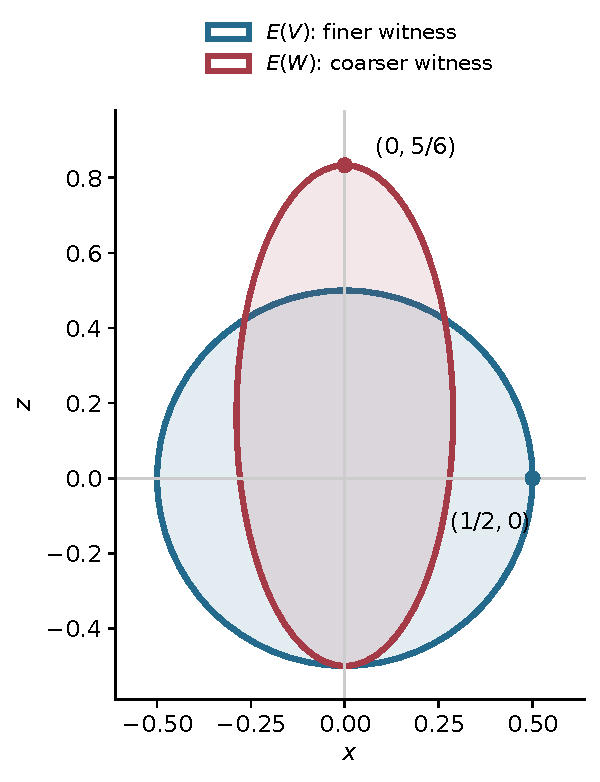
\includegraphics[width=.52\linewidth]{figures/class_c_incomparability.pdf}
\caption{An $xz$ section of the two Class C ellipsoids. The spherical witness $V$ is strictly finer than $W$, but neither ellipse contains the other. The marked points certify both failures of containment.}
\end{figure}

\subsection{Unbounded reversal of ellipsoid volume}

The failure of geometric monotonicity cannot be repaired by replacing containment with volume. For $0<\delta\leq1/8$, define
\[
 V_\delta=\tfrac14[\II+(1-\delta)\XX+\delta\YY+\delta\ZZ],
 \qquad W_\delta=\tfrac34V_\delta+\tfrac14\proj{\phi^-}.
\]
Both are canonical right-handed Class C witnesses. Their positive correlation diagonals are respectively
\[
 (1-\delta,\delta,\delta),\qquad
 \left(\frac{2-3\delta}{4},\frac{1+3\delta}{4},\frac{1+3\delta}{4}\right).
\]
The only negative Bell eigenvalue of $V_\delta$ is $-\delta/4$; that of $W_\delta$ is $-3\delta/16$. Their partial-transpose spectra, in Bell order, are respectively
\[
 \left(\frac{2+\delta}{4},\frac{\delta}{4},\frac{2-3\delta}{4},\frac{\delta}{4}\right),\qquad
 \left(\frac{8+3\delta}{16},\frac{2+3\delta}{16},\frac{4-9\delta}{16},\frac{2+3\delta}{16}\right).
\]
All entries are positive in the stated interval. The state
\[
 \rho=\tfrac78\proj{\psi^-}+\tfrac18\proj{\phi^-}
\]
has expectations $-\delta/8$ and $(1-3\delta)/32$, proving strict fineness of $V_\delta$ over $W_\delta$.

Their volume ratio, with the common ball-volume factor cancelled, is
\[
 \frac{\operatorname{vol}\E(W_\delta)}{\operatorname{vol}\E(V_\delta)}
 =\frac{(2-3\delta)(1+3\delta)^2}{64(1-\delta)\delta^2}
 \longrightarrow\infty\qquad(\delta\downarrow0).
\]
Thus the finer witness can have an arbitrarily smaller ellipsoid, even with positive chirality and Class C fixed. This family is verified algebraically in the accompanying symbolic checks; it is not included among the claimed Lean theorems.



\section{Planar targets, admissibility, and practical decision rules}

For $0<a,b\leq1$ and $a+b>1$, the witness
\[
 D_{a,b}=\tfrac14(\II+a\XX+b\YY)
\]
has a rank-two ellipsoid with semiaxes $a,b,0$. Its Bell eigenvalues are
\[
 (1+a-b)/4,\quad(1-a+b)/4,\quad(1+a+b)/4,\quad(1-a-b)/4.
\]
Its partial transpose is another witness of the same ellipse, so it is Class D. At $a=b=3/4$ this is a radius-$3/4$ disk strictly inside the Bloch ball, with spectrum $\{1/4,1/4,5/8,-1/8\}$. Every witness representing the whole disk is relatively optimal. This supplies a concrete strictly interior planar instance of the singular-target proof.

For any proposed target $c_*+A\B\subseteq\B$ of rank at least two, choose the orientation convention used in Part~I and form
\[
 W_*=(L\otimes\id)(\Phi^\Gamma).
\]
The target is admissible exactly when $W_*$ fails to be positive semidefinite. In full rank, an admissible target is Class C when $W_*^\Gamma\succeq0$ and Class D otherwise. In rank two, admissible targets are Class D. This is a finite matrix test, with the initial containment of the target in the Bloch ball checked independently. It avoids treating the word ``admissible'' as a purely pictorial condition.

The resulting workflow is explicit:
\begin{enumerate}
\item Extract the Pauli data $a,b,T$ and certify witness validity.
\item Check target admissibility and rank. If the rank is at most one, there are no witnesses in its containment set.
\item Certify containment using the support constraints and the S-lemma matrix, or the support-function condition.
\item Test the polynomial equalities and determinant sign in \eqref{eq:polynomial-optimality}.
\item If the witness is not optimal, solve \eqref{eq:sdp-primal}. The exact optimizer has rank one; numerical rank is only a diagnostic.
\item Certify the resulting positive remainder. When available, a matching dual certificate proves minimum trace exactly.
\end{enumerate}

The mathematical existence proof and the implementation serve different purposes. The proof handles singular and exceptional cases exactly. The numerical solver makes examples accessible and can suggest rational certificates, but its floating-point output is never substituted for the mathematical or Lean proofs.
